%%%% IACR Transactions TEMPLATE %%%%
% This file shows how to use the iacrtrans class to write a paper.
% Written by Gaetan Leurent gaetan.leurent@inria.fr (2020)
% Public Domain (CC0)


%%%% 1. DOCUMENTCLASS %%%%
\documentclass[journal=tosc,submission]{iacrtrans}
%%%% NOTES:
% - Change "journal=tosc" to "journal=tches" if needed
% - Change "submission" to "final" for final version
% - Add "spthm" for LNCS-like theorems


%%%% 2. PACKAGES %%%%
\usepackage{lipsum} % Example package -- can be removed
\usepackage{blt}
\usepackage{tabularx}
\usepackage{graphicx}
\usepackage{xcolor}
\usepackage{url}


%%%% 3. AUTHOR, INSTITUTE %%%%
\author{Maximilian Heim}
\institute{
  University Albstadt-Sigmaringen, Albstadt, Germany, \email{MaximilianHeim@protonmail.com}
}
%%%% NOTES:
% - We need a city name for indexation purpose, even if it is redundant
%   (eg: University of Atlantis, Atlantis, Atlantis)
% - \inst{} can be omitted if there is a single institute,
%   or exactly one institute per author


%%%% 4. TITLE %%%%
\title{Return Oriented Programming}
%%%% NOTES:
% - If the title is too long, or includes special macro, please
%   provide a "running title" as optional argument: \title[Short]{Long}
% - You can provide an optional subtitle with \subtitle.

\begin{document}

\maketitle


%%%% 5. KEYWORDS %%%%
\keywords{ROP \and Return Oriented Programming \and Buffer Overflow \and Binary Exploitation}


%%%% 6. ABSTRACT %%%%
\begin{abstract}
  In this paper we introduce the concept of Return Oriented Programming, how to apply it, how to protect against it and show a concrete attack.
\end{abstract}


%%%% 7. PAPER CONTENT %%%%
\section{Introduction}
BIBLIOGRAFIE NICHT VERGESSEN
Return Oriented Programming is a type of buffer overflow attack that has been published in 2007 and ever since has become a widely known buffer overflow technique. It has been developed to circumvent the NX-BIT protection that protects the stack from being executed. At the time of writing this paper modern techniques like Stack Carnaries and ASLR prevent these attacks from being practical but there are millions of running systems using old hard-, firm- and software that is possibly vulnerable to these kinds of buffer overflow attacks. Return Oriented Programming is based on chaining return addresses to code just before a return and therefor allowing almost arbitrary code segments to be chained.


\section{Gadgets}
\label{sec:main}
\paragraph{Introduction}
Gadgets are code segments that sit before a \Verb+ret+ instruction, that is an instruction that uses the address on the stack to return to a previous stack frame and therefor a previous level in the call hierarchy. This means we can arbitrarily chain these gadgets and achieve arbitary code execution if we find gadgets for our purpose.

\paragraph{How to find Gadgets}
A gadget can be found by searching for \Verb+0xC3+ Bytes in the program. The instructions before then represent the code we can use, for that we need the address of the gadget. We could do this manually using tools like \Verb+objdump+, \Verb+hexdump+ or use one of the many tools available, to name a few there is \Verb+ropper+, \Verb+ROPgadget+ and \Verb+pwntools+. For this paper i will be using \Verb+ROPgadget+ since i found it easy to use and fast. Using the following command~\cref{dumpallgadgets} under Linux we can dump all gadgets to a file and search in it using regular expressions, \Verb+ROPgadget+ can be found in most package managers or can be downloaded directly from \url{https://github.com/JonathanSalwan/ROPgadget}.
\paragraph{Finding gadgets using ROPgadget}
\bltCommand{ropcommand.sh}{Dumping all gadgets into a file}{dumpallgadgets}
Using this command produces an output with results similar to this.
\bltResult{dumppick}{Output of ROPgadget}{outputropgadget}
These are only 10 Lines out of the 8244 lines found by the tool though and i purposefully filtered out some good and bad ones for demonstration. It is clearly visible that many candidates for ROP can be found, even in a file with a relatively small size of 72 kB. Though most of these gadgets are not all that useful because they often modify a lot of registers, possibly messing up the desired state or use a fixed return address. In most cases we can find suitable candidates using regular expressions though, this will be demonstrated later in this section.
\paragraph{Overview of powerful gadgets}
\paragraph{pop}
Pop allows us to write arbitrary values into registers. For that we search for a \Verb+pop <reg>+ instruction inside our gadgets, in the payload we can then place the value after the address of the pop instruction. If we can not find a suitable gadget we can try to get creative and achieve the desired state another way. If for example we want to write some value into ecx we could use something like this: \Verb+xor ecx, ecx ; pop eax ; xor ecx, eax+. Provided that we have these gadgets available.
\paragraph{mov}
Mov allows us to write arbitrary values into memory. For that we search for a \Verb+mov dword ptr [<reg1>], <reg2>+ instruction inside our gadgets, we can then, in combination with two pops write arbitrary values at arbitary memory locations, we could use something like this to accomplish that: \Verb+pop ecx ; pop eax ; mov dword ptr [eax], ecx+
\paragraph{arithmetics, boolean algebra}
Arithmetic operations like \Verb+add+, \Verb+sub+, \Verb+inc+, \Verb+xor+, \Verb+or+, and can be useful to bring registers into our desired state. For that we search for the corresponding gadget with the required operands. For example \Verb+xor+ can be used to clear a register or copy its contents. It often occurs in the following forms: \Verb+xor eax, eax+ or \Verb+xor eax, edx+. The first case clears the register since \Verb+xor+ computes a non-equivalence, formally $a \oplus a = 0$ and the second one copies the value of the 2nd operand into the 1st operand when the target register is \Verb+0x00+ since \Verb+0x00+ is the neutral element of the \Verb+xor+ operation, formally $a \oplus 0 = a$.
\paragraph{int 0x80}
\Verb+int+ stand for an interrupt, the interrupt \Verb+0x80+ causes a system call to be executed. System calls are kernelspace programs/operations that require higher privileges than what is available in a userspace program. Examples for system calls include io and \Verb+execve+ which allows to execute arbitary programs. In combination with \Verb+pop+, \Verb+mov+ and other instructions we can specify the concrete system call. One of the most powerful system calls for blackhats is bash since it allows permanently implementing malware or gain insight into files, it can be called with the argument \Verb+/bin/sh+.
\subsection{Filtering the gadgets}
\paragraph{Introduction}
In order to find the gadgets we want we can use the tools directly or we can use regular expressions. In order to make this paper more general and easy to replicate i will be using regular expressions to find the desired gadgets.
\paragraph{Gadgets and their corresponding Regular Expression}
The following table describes what regex we can use to find the gadgets needed for the attack.

\begin{itemize}
\item pop edx  $\rightarrow$ \bltRegex{\^{}.\{0,20\}pop edx.\{0,20\}ret\\n}

\item int 0x80  $\rightarrow$ \bltRegex{\^{}.\{0,20\}int 0x80} 

\item xor eax, eax  $\rightarrow$ \bltRegex{\^{}.\{0,20\}xor eax, eax.\{0,20\}ret\\n} 
\end{itemize}

for all of these regular expressions i was able to find at least a few suitable candidates. If there are no results the amount of possible characters before or after the gadget can be increased until results show up. It is however desirable to have gadgets with as few and noninterfering instructions as possible, if this is accomplished we can almost use the instructions we found like in assembly. Gadgets which do multiple things at once however can mess up the desired state and break the payload so it is important to thoroughly analyze the gadgets before using them.

\section{Theory}
\subsection{Stack}
\begin{figure}[h]
  \centering
  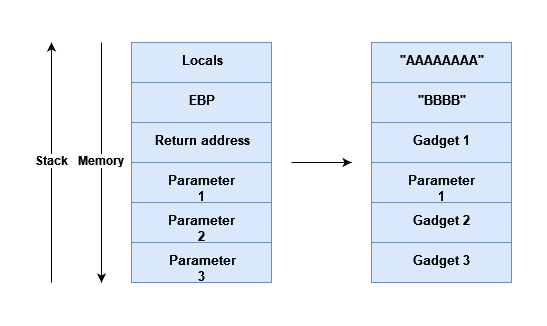
\includegraphics[width=0.65\textwidth]{stackropoffsec.png}
  \caption{The stack when injecting the payload}
  \label{fig:mesh1}
\end{figure}
\subsection{ROP Chain}

\section{Attack}
\label{sec:attack}
\subsection{Target Program}
\paragraph{Target Program}
The following program is the target of our attack, it uses a command line argument to provide the payload and \Verb+strcpy+ for the buffer overflow, overwriting the return address after the 8 Byte buffer. Using vulnerable input functions also works though.
\bltCode{vuln.c}{c}{The Target Program}{thetargetprogram}

\paragraph{Compilation}
We use the following command to compile the target program
\bltCommand{compilation.sh}{The compliation command}{thecompilationcommand}

\subsection{Phases of developing the attack}
\paragraph{Phases}
The attack consists of several phases
\begin{enumerate}
  \item Specify concrete goal with required program state and instructions
  \item Generate desired list of instructions and arguments (abstract payload)
  \item Extract gadgets using tools
  \item Search gadgets for instructions
  \item Generate payload using the gadgets according to the the abstract payload while making sure gadgets dont interfere with our desired program state. This step can be done using Python which we will show in a later section~\cref{howtopack}
  \item Insert payload into target
\end{enumerate}

\paragraph{Goal and abstract payload}
After specifying the goal and possibly simplifying it we have to write a list of instructions and arguments that achieve the goal, for this its favorable to directly use the format of the final payload except for using instructions instead of addresses as this will then allow to simply insert the found gadgets into this abstract payload.
\paragraph{Extract and search gadgets}
After extracting the gadgets using one of the above mentioned methods we can search for gadgets

As described above you should 

\paragraph{struct.pack}
\Verb+struct.pack+ is a Python function that allows to easily generate our desired payload from the raw bytes. Bash then allows to directly pipe the generated payload into our target. In order to generate the payload we first have to fill the buffer and override the EBP with arbitary values as seen in line 2~\cref{howtopack}. This is usually done using easily recognizable characters, using the letter \Verb+A+ for this is common. It has the hex value \Verb+0x41+, doing this allows then to spot the buffer in a debugger like \Verb+gdb+. So in this example we fill the buffer with 8 \Verb+A+'s and 4 \Verb+B+'s. After that it is time to insert the addresses of the gadgets and the arguments. This is done by calling pack with the double word (64 Bit) while specifying the endianness, converting that to a string and adding it to the string as seen in line 3~\cref{howtopack}. After the whole payload has been generated we can print it and use the output directly for running the buffer overflow attack as mentioned above.
\bltCode{pack.py}{python}{How to use struct.pack}{howtopack}
\section{Results}
\paragraph{Attack}
After injecting the generated payload from \cref{sec:attack} as a command line argument the program opened a shell from which we can use privilege escalation techniques in order to completely compromise the system. The only compiler options that had to be activated were PIE and stack canaries. It is likely that there are systems still in use today which are vulnerable to this kind of attack. Since it allows almost arbitrary code execution it is very important to identify these devices and patch or replace them.
\paragraph{ASLR}
The information about wether or not ROP can be applied to systems with ASLR enabled is inconsistent. In the run with PIE and stack canaries disabled the attack still worked even with \Verb+/proc/sys/kernel/randomize_va_space+ set to \Verb+2+, meaning full randomization of the different segments like header, libraries and stack. This is probably due to PIE
\section{Protection}
Luckily we had to disable several security mechanisms to make this attack possible, especially 

\section{Discussion}
Sources:
https://www.exploit-db.com/docs/english/28479-return-oriented-programming-(rop-ftw).pdf
%%%% 8. BILBIOGRAPHY %%%%
\bibliographystyle{alpha}
\bibliography{abbrev3,crypto,biblio}
%%%% NOTES
% - Download abbrev3.bib and crypto.bib from https://cryptobib.di.ens.fr/
% - Use bilbio.bib for additional references not in the cryptobib database.
%   If possible, take them from DBLP.
\end{document}
